\section{Analyse der statischen Ist-Architektur}

\subsection{Reverse Engineering}
Da die Ist-Architektur des FreeDesign-Editors kaum dokumentiert war, musste die aktuelle Architektur zunächst rekonstruiert werden. 
Dies wird als \emph{Reverse Engineering} bezeichnet und hat, laut der Definition von Chikofsky und Cross (\citeyear[S. 13-17]{Chikofsky1990}), zwei Ziele: 
\begin{itemize}
    \item Die Darstellung des Softwaresystem in einer abstrakten Form. 
    \item Die Identifikation der Komponenten eines Softwaresystems und ihre Beziehungen untereinander. 
\end{itemize}
Das Reverse-Engineering der Ist-Architektur de FreeDesign-Editor bezieht sich auf den Projektzustand vom 11. Januar 2020. 
% Für das Reverse Engineering der statischen Ist-Architektur stand im Fokus, eine Grundlagen für den Entwurf einer statischen Soll-Architektur zu erstellen.
% Daher konzentriete sich die Reverse-Engineering auf das identifizieren von Baustein aus denen der FreeDesign-Editor besteht und auf denen die Soll-Architektur basieren kann. 
% Den Bausteinen wurden weiterhin Bestandteile des Quelltextes der aktuellen Implementation zugeordnet. 

\subsection{Darstellung des Softwaresystems}
Das Ziel der Darstellung des Softwaresystems war, es in einer Form darzustellen, dass sich Komponenten identifizieren lassen sowie ihre Integration in der Ist-Architektur. 

\subsubsection{Das {dependency-cruiser}-Werkzeug}
Das Reverse Engineering kann durch den Einsatz von Analyse-Werkzeugen unterstützt werden, wobei üblicherweise ein einzelnes Werkzeug nicht alle Analyse-Aufgaben übernehmen kann  \autocite[vgl.][381]{Bass2013}.  

Für die Visualisierung der Ist-Architektur wurde das Werkzeug \emph{dependency-cruiser}, welches von Sander Verweij entwickelt und unter \url{https://github.com/sverweij/dependency-cruiser} veröffentlicht wurde, in der Version v9.22.0 eingesetzt. 
Das Werkzeug untersucht das Quellentextverzeichnis eines TypeScript-Projektes und visualisiert die Struktur des Quelltext als Abhängigkeitsgraph. Weiterhin können Regeln für die Abhängigkeiten der Komponenten angelegt werden, die durch das Werkzeug validiert, Verstöße gekennzeichnet und als Report ausgeben werden \autocite[vgl.][]{Verweij:Dependency}. 

Das \emph{dependency-cruiser}-Werkzeug ist ein Programm für die Kommandozeile, welches mit unterschiedlichen Argumenten aufgerufen werden kann \autocite[vgl.][]{Verweij:CLI}.

\subsubsection{Konfiguration des {dependency-cruiser}-Werkzeug}
Für alle Analysen mit dem dependency-cruiser-Werkzeug wurde die selbe Konfigurationsdatei angelegt, welche im Anhang unter \emph{dependency-cruiser-konfiguration.json} enthalten ist. Diese wurde beim Aufruf des Programms durch die Angabe des Argumentes \lstinline|--config| eingebunden.
\begin{lstlisting}[language={sh},label=depcruise-config, caption=Aufruf des \emph{dependency-cruiser} mit eingebundener Konfigurationsdatei]
    npx depcruise --config dependency-cruiser-konfiguration.json src
\end{lstlisting}
Die Konfigurationsdatei liegt im JSON-Format vor. 

Das JSON-Format ist ein, sprachunabhängiges Format zum Austausch von Informationen, welches auf strukturierten Text basiert. Der Text ist ein serialisiertes Objekt oder Array, deren Werte vom Datentyp Objekt, Array, Nummer oder eine Zeichenkette sein können. Weiterhin sind die Literale \lstinline|null|, \lstinline|true| und \lstinline|false| valide Wertzuweisungen \autocite[vgl.][]{JSON:Einführung}.  

Das Konfigurationsdatei besteht aus einem JSON-Objekt mit den drei Eigenschaften \lstinline|forbidden|, \lstinline|allowed| und \lstinline|options|.

% options
Der Eigenschaft \lstinline|options| ist ein Objekt zugewiesen mit den Eigenschaften 
\lstinline|tsConfig|, 
\lstinline|webpackConfig|, 
\lstinline|reporterOptions| und 
\lstinline|exclude|. Die Eigenschaften \lstinline|tsConfig| und \lstinline|webpackConfig| enthalten Konfigurationsinformation zum TypeScript-Projekt. Über die Eigenschafte reporterOptions konnte Einfluss auf das Ausehen der Abhängigkeitsgraphen genommen werden. Für Eigenschaft \lstinline|exclude| wurde ein Array mit Pfadangaben, die von der Analyse ausgeschlossen werden sollten, angelegt. Dies betraf Abhängigkeiten zu externen Javascript-Bibleotheken, die für die interne Architektur keine Rolle spielen sowie Daten für Unit-Tests und CSS-Dateien. 

% forbidden & allowed
Die Eigenschaften \lstinline|forbidden| und \lstinline|allowed| sind jeweils vom Datentyp Array und enthalten die Regeln zur Validierung der Abhängigkeiten zwischen den Quelltextkomponenten. 
In beiden Arrays werden Abhängigkeiten durch eine Objektstruktur angeben, welche die Eigenschaften \lstinline|from| und \lstinline|to| enthält. Beide Eigenschaften einthalten wiederum die Eigenschaft \lstinline|path|, welcher entweder ein Dateipfad-Fragment als Zeichenkette oder ein Array aus Dateipfad-Fragmenten zugewiesen werden kann. Die Struktur wird anhand eines Beispiels in Listing \ref{depcruise-example} illustriert.

\begin{lstlisting}[language={sh}, label=depcruise-example, caption=Beispiel einer Abhängigkeitesrelation]
{
    "from": { "path": "^src/services" },
    "to": { "path": [
        "^src/core",
        "^src/store",
        "^src/actions/types/ApiActionTypes.ts",
        "^src/actions/types/ProductApiActionTypes.ts",
        "^src/actions/types/GuiActionTypes.ts"
    ]}
},
\end{lstlisting}
Das Beispiel stammt aus dem \lstinline|allowed|-Array und erlaubt somit, dass Quelltext der innerhalb des Ordners \lstinline|src/services| liegt, auf Quelltext innerhalb der in \lstinline|to| angeben Pfade zugreifen darf. 
Somit ist beispielsweise die Importangabe \newline  
\glqq\lstinline|import ApiRoutes from '../../core/api/ApiRoutes';|\grqq \newline
innerhalb der Datei \lstinline|src/services/designService/CustomerDesignService.ts| valide.

Zunächst wurden Abhängigkeiten, für die innerhalb des Teams Konsens besteht, dass es sie grundlegend nicht geben darf, in das \lstinline|forbidden|-Array eingetragen. Während der Analyse der Ist-Architektur wurden die bestehenden Abhängigkeiten überprüft und alle Abhängigkeiten die für valide befunden wurden in das \lstinline|allowed|-Array aufgenommen. Da es für die Abhängigkeiten nur lose, mündlich kommunizierte Regeln gab, konnten nur wenige Einschränkungen der Abhängigkeiten getroffen werden.  

Das \lstinline|forbidden|-Array wurde außerdem durch die Einträge 
\lstinline|no-orphans| und \lstinline|no-circular| ergänzt.

Der Eintrag \lstinline|no-orphans| dient zum Aufdecken von ungenutzten Quelltext was für die Entwicklung der Soll-Architektur wichtig war.

Mit Hilfe der Option \lstinline|no-circular| konnten zyklische Abhängigkeiten aufgedeckt werden.

Anlehnend an Lilienthal (\citeyear[vgl.][88 - 90]{Lilienthal2019}) greifen bei zyklischen Abhängigkeiten Komponenten gegenseitig aufeinander zu und bedingen sich somit gegenseitig. 

\begin{figure}[H]
    \centering
    \caption{Beispiele für Abhängigkeiten basierend auf Lilienthal}
    \label{fig:exampleCircular}
    \begin{subfigure}[b]{.3\textwidth}
        \centering
        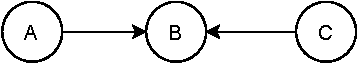
\includegraphics[width=.9\textwidth]{diagrams/Methoden/Circular-Example-C.pdf}
        \caption{ohne Zyklus}
        \label{fig:circularA}
    \end{subfigure}
    %\qquad
    \begin{subfigure}[b]{.3\textwidth}
        \centering
        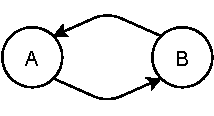
\includegraphics[width=.6\textwidth]{diagrams/Methoden/Circular-Example-A.pdf}
        \caption{mit Zyklus}
        \label{fig:circularB}
    \end{subfigure}
    %\qquad
    \begin{subfigure}[b]{.3\textwidth}
        \centering
        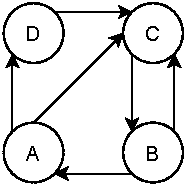
\includegraphics[width=.5\textwidth]{diagrams/Methoden/Circular-Example-B.pdf}
        \caption{Zyklusgruppe}
        \label{fig:circularC}
    \end{subfigure}
\end{figure}
In Abbildung \ref{fig:circularA} sind zwei zyklusfreie Abhängigkeit illustriert, wobei A und B auf C zugreifen. Somit sind A und B abhängig von C. Eine Änderung an C hat Einfluss auf A und B, jedoch hat eine Änderung in A oder B keinen Einfluss auf C. Dadurch sind Abhängigkeiten leicht verständlich und problemlos Erweiterbar. 
Auch lässt sich B isoliert von A und C testen. Für Tests von A und C kann B einfach simuliert werden.

Treten hingegen Zyklen in den Abhängigkeiten auf, wie in Abbildung \ref{fig:circularB} und \ref{fig:circularC} illustriert, verringert sich die Verständlichkeit des Quelltextes und er lässt sich nur schwer ändern. Bezogen auf Abbildung \ref{fig:circularB}, kann ein Änderung in A eine Änderung B zu folge haben. Die Änderung in B kann wiederum einen Änderung in A notwendig machen. Somit können Änderung eine rückkoppelnde Wirkung haben.

Die so auf gedeckten Zyklen zeigten Potentiale zur Verbesserung der Ist-Architektur und musste bei der Entwicklung der Strategie zur Migration in die Soll-Architektur beachtet werden.

\subsubsection{Erzeugung eines Validierungsreport}
Mit dem in Listing \ref{depcruise-report} angeben Kommando wurde auf Basis der Regeln, die in der Konfigurationsdatei hinterlegt wurden, ein Report erstellt.
Der Report enthält eine Liste aller Verstöße gegen die angegebenen Regeln.
\begin{lstlisting}[language={sh}, label=depcruise-report, caption=Erzeugung eines Validierungsreport]
npx depcruise --config dependency-cruiser-konfiguration.json -T err-html src -f Validierungsreport.html
\end{lstlisting}

\subsubsection{Erzeugung der Visualisierungen}
Durch das nutzen verschiedener Argumente konnten unterschiedliche Darstellungen der Ist-Architektur mit unterschiedlichem Fokus erzeugt werden. 

Zunächst wurde die Beziehungen der Quelltextkomponenten auf der obersten Ordnerebene visualisiert und analysiert. 
Hierzu wurde das Werkzeug mit folgende Argumenten aufgerufen:

\begin{lstlisting}[language={sh}, label=depcruise-overview, caption=Kommando zur Erzeugung der Visualisierung der obersten Ordnerebene]
npx depcruise --config dependency-cruiser-konfiguration.json -T archi src | dot -T svg > Projektuebersicht.svg
\end{lstlisting}

Für das Argument \lstinline|--output-type|, welches den Typen der Ausgabe angibt, wurde die Kurzform  \lstinline|-T| genutzt. Mit Hilfe des Typen \lstinline|archi| können zusammenfassende Übersichten der Abhängigkeiten erstellt werden, in den lediglich die oberster Ordnerebene dargestellt werden \autocite[vgl.][]{Verweij:Options}.
Der so erzeugte Abhängigkeitsgraph wurde anschließend als SVG-Datei gespeichert. 
\newline
Die Visualisierung sämtlicher Abhängigkeiten der Software ergibt einen sehr umfangreichen und unübersichtlichen Graphen. Daher wurden mehrere Graphen erzeugt, die sich auf die Hauptaufgaben der Software beziehen:
\paragraph{Die Produktpräsentation} gehört zu den wichtigsten Aufgaben des FreeDesign-Editors. 
Der dafür verantwortliche Quelltext ist im Ordner 
\lstinline|src/components/pagePresenter| enthalten. Mit dem unter Listing \ref{depcruise-page-presenter} angegebenen Kommando, konnten visualisiert werden, von welchem Quelltextkomponente die Produktpräsentation abhängig ist. 
\begin{lstlisting}[language={sh}, label=depcruise-page-presenter, caption=Erzeugung der Visualisierung der Abhängigkeiten für die Produktpräsentation]
npx depcruise --config dependency-cruiser-konfiguration.json -T dot
  src/components/pagePresenter | dot -T svg > Produktpraesentation.svg
\end{lstlisting}

\paragraph{Die Designpräsentation} gehört ebenfalls zu den zentralen Aufgaben des FreeDesign-Editors. Die Designpräsentation ist entkoppelt von der Produktpräsentation und wird dieser lediglich übergeben, wodurch das Design innerhalb der Produktpräsentation dargestellt werden kann.
Der für Designpräsentation verantwortliche Quelltext ist im Ordner \lstinline|src/components/pagePresenter| hinterlegt. Die Quelltextkomponente auf die die Designpräsentation zugreif konnten mit folgendem Kommando visualisiert werden:  
\begin{lstlisting}[language={sh}, label=depcruise-design-presenter, caption=Erzeugung der Visualisierung der Abhängigkeiten für die Designpräsentation]
npx depcruise --config dependency-cruiser-konfiguration.json -T dot 
  src/components/designPresenter | dot -T svg > Designpraesentation.svg
\end{lstlisting}

\paragraph{Das Editieren von Designs} ist die Kernaufgabe des FreeDesign-Editors. 
An dieser Aufgaben sind sehr viele Quelltextkomponenten des Editors beteiligt, die ausgehen vom Redux-Container \lstinline|Stage.tsx| zusammearbeiten. Die Datei \lstinline|Stage.tsx| ist im Ordner \lstinline|src/containers/stage| hinterlegt, deren Abhängigkeiten durch das folgende Kommando visualisiert wurden.
\begin{lstlisting}[language={sh}, label=depcruise-design-edit, caption=Visualisierung der Abhängigkeiten für den Quelletext zum editieren des Designs]
npx depcruise --config dependency-cruiser-konfiguration.json -T dot  
  src/containers/stage | dot -T svg > Designeditieren.svg      
\end{lstlisting}
Da das Editieren von Designs von sehr vielen Quelltextkomponenten abhängig ist und dadurch der Graph sehr umfangreich ist, wurde eine weitere kompakte Darstellung erzeugt. Hierzu wurde das Argument \lstinline|--collapse| angewandt, welches eine Graph der beteiligten Ordner erzeugt \autocite[vgl.][]{Verweij:CLI}. 
\begin{lstlisting}[language={sh}, label=depcruise-design-edit-compact, caption=Visualisierung der Abhängigkeiten für den Quelletext zum editieren des Designs]
npx depcruise --config dependency-cruiser-konfiguration.json --collapse 
  ".*/" -T dot src/containers/stage | dot -T svg > 
  Designeditieren-kompakt.svg
\end{lstlisting}

\paragraph{Die grafische Oberfläche} des FreeDesign-Editors
enthält, neben dem Redux-Container Stage, eine Reihe weitere Elemente. Eine Übersicht der Elemente und der Abhängigkeiten wurden mit dem, in Listing \ref{depcruise-gui} angeben, Kommando erzeugen. Da sich der FreeDesign-Editor aus Redux-Container-Elementen zusammensetzt, die auf React-Komponenten, den Redux-State und Redux-Actions zugreifen, konnte die Analyse basierend auf dem Ordner \lstinline|src/containers| erfolgen. Da die Visualisierung sonst zu umfangreich während, wurde \lstinline|--collapse| genutzt sowie der Redux-Container Stage mit dem Argument \lstinline|--do-not-follow| ausblendet.

\begin{lstlisting}[language={sh}, label=depcruise-gui, caption=Visualisierung der Zusammenhänge der grafischen Elemente des Editors]
npx depcruise --config dependency-cruiser-konfiguration.json 
  --do-not-follow "^src/containers/stage" --collapse ".*/" -T dot 
  src/containers | dot -T svg  > 
  Grafische-Oberflaeche.svg
\end{lstlisting}

\paragraph{Das Konvertieren von Adobe-Illustrator-Dateien} in FreeDesign-Designs, welches als Kommandozeilenprogramm für den, in Abschnitt \ref{sect:Integrationsprozess_Designvorlagen} beschrieben, Integrationsprozess bereitgestellt wird, ist ebenfalls ein Teil des FreeDesign-Projektes. 
Das Kommandozeilenprogramm wird durch die Datei \lstinline|src/draftImporterCli.ts| umgesetzt, der Abhängigkeiten durch folgendes Kommando visualisiert werden konnten.
\begin{lstlisting}[language={sh}, label=depcruise-draft-import, caption=Visualisierung der Abhängigkeiten des Programms zum Import der AI-Dateien]
npx depcruise --config dependency-cruiser-konfiguration.json -T dot 
  src/draftImporterCli.ts | dot -T svg > AI-Import.svg
\end{lstlisting}

\paragraph{Das Konvertieren von FreeDesign-Designs in SVG-Dateien} als Basis für das Erstellen der Vorschaubilder ist ebenfalls ein Teil des, in Abschnitt \ref{sect:Integrationsprozess_Designvorlagen} beschrieben, Integrationsprozess.  
Das Kommandozeilenprogramm für diesen Schritt wurde im Ordner \lstinline|src/designToSvgCLI| umgesetzt. Die Abhängigkeit wurden mit folgendem Kommando visualisiert.
\begin{lstlisting}[language={sh}, label=depcruise-design-to-svg, caption=Visualisierung des Kommandozeilenprogramms designToSvgCLI]
npx depcruise --config dependency-cruiser-konfiguration.json -T dot 
  src/designToSvgCLI | dot -T svg > SVG-Konvertierung.svg
\end{lstlisting}

% Das Werkzeug dependency-cruiser unter einer MIT-Linzenz zu Verfügung gestellt, welche eine kostenfreien Nutzung garantiert \autocite[vgl.][]{Verweij:License}. 


\subsection{Identifikation von Bausteinen}
Starke und Hruschka bezeichnen die Komponenten eines Softwaresystems als Bausteine, die miteinander in Beziehungen stehen \autocite[vgl.][24]{Starke2011}. Diese Bezeichnung wird auch in der vorliegenden Diplomarbeit angewendet, um einer Verwechselung zwischen Softwarebausteinen und React-Komponenten vorzubeugen.

Mit Hilfe der Abhängigkeitsgraphen wurden die Bausteine, aus denen der FreeDesign-Editor besteht, identifiziert. 

Um Fragmente des Quelltextes den Bausteinen zuzuordnen, wurde ein kleines Werkzeug entwickelt, welches das Quellenverzeichnis rekursiv durchsucht. Zum einen sucht es nach Dateien mit der Bezeichnung \glqq\lstinline|_component.md|\grqq{} und zum anderen, innerhalb der Quelltextdateien, nach der Textphrase \glqq\lstinline|// @component{BAUSTEINNAME}|\grqq{}. 
Mit Hilfe der \lstinline|_component.md|-Dateien, deren einziger Inhalt der Name eines Bausteins ist, kann der Inhalt eines bestimmten Verzeichnisses einem Baustein zugeordnet werden. Einzelne Quelltextdateien können mit der Textphrase \glqq\lstinline|// @component{BAUSTEINNAME}|\grqq{} Bausteinen zugeordnet werden. Die Textphrase kann auch mehrfach innerhalb einer Datei enthalten sein, wodurch es möglich ist, eine Datei mehreren Bausteinen zuzuordnen. 

Das Ergebnis der Analyse ist eine tabellarische Zuordnung von Bausteinen zu Quelltext-Fragmenten in Form einer HTML-Datei. 
Der Entwurf der Soll-Architektur konnte somit auf der Auflistung der Bausteine basieren. Die Zuordnung der Quelletext-Fragmente der aktuellen Implementation, half dabei die Beziehungen zwischen den Bausteinen zu ordnen und eine Mirgrationsstrategie zu entwerfen.

Das Werkzeug ist im Anhang unter \emph{Komponentenzuordnung} enthalten.